\section{Induced Topologies} 

\subsection{Initial and Final Topologies} 

  We have seen some examples of how to create topologies. They can be created without any assumptions on the set, such as the discrete, indiscrete, and the cofinite topologies. More often, we want to consider how a certain structure like the order or a metric induces a topology. Now, we will consider how \textit{functions} can induce a topology. The uniqueness of such induced topologies is called the \textit{universal property}. 

  \begin{definition}[Initial Topology]
    Given a space $X$ and a family of topological spaces $\{Y_\alpha\}_{\alpha \in A}$ 
    \begin{equation}
      f_i : X \rightarrow (Y_\alpha, \T_\alpha)
    \end{equation} 
    the \textbf{initial topology} on $X$ is the coarsest topology $\T$ on $X$ s.t. that each 
    \begin{equation}
      f_i (X, \T) \rightarrow (Y_\alpha, \T_\alpha)
    \end{equation}
    is continuous. 
  \end{definition}

  \begin{definition}[Final Topology]
    Given a space $Y$ and a family of topological spaces $\{X_\alpha\}_{\alpha \in A}$ 
    \begin{equation}
      f: (X, \T_\alpha) \rightarrow Y
    \end{equation}
    the \textbf{final topology} on $Y$ is the finest topology $\T$ on $Y$ s.t. each 
    \begin{equation}
      f: (X, \T_\alpha) \rightarrow (Y, \T)
    \end{equation}
    is continuous. 
  \end{definition}

  Note that it makes sense to talk about the coarsest topology on the domain and the finest topology on the codomain. If it were the other way around, i.e. the finest topology on the domain, then the initial topology on $X$ would be the discrete topology, making every function defined on $X$ continuous. In the same logic, the coarsest topology on $Y$ would trivially be the trivial topology, making all $Y$-valued functions continuous. With these current definitions, if $\T_Y$ is too fine (e.g. if $\T_Y = 2^Y$), then the open sets of $\T_Y$ would be too fine and therefore would have a preimage that may not be open in $X$. 

\subsection{Subspace Topology} 

  The reason we want to do this is because we want to think of $Y$ as its own entity, independent of $X$. 

  \begin{definition}[Subspace Topology]
    Given topological space $X$ and subspace $Y \subset X$, the \textbf{subspace topology} on $Y$ is defined in the equivalent ways. 
    \begin{enumerate}
      \item It is the initial topology on the subspace $Y$ with respect to the inclusion map $\iota: Y \rightarrow X$. 
      \item It is the topology consisting of $X$-open sets intersection $Y$.
      \begin{equation}
        \T_Y = \{(U \cap Y) \subset Y \mid U \in \T_X\}
      \end{equation}
      We can also say that $A \subset Y$ is closed in $Y$ iff it is the inersection of $Y$ with a closed set of $X$. 
    \end{enumerate}

    \begin{figure}[H]
      \centering
      \begin{subfigure}[b]{0.48\textwidth}
        \centering
        \begin{tikzpicture}
          % Draw the x and y axes in gray
          \draw[gray] (-3,0) -- (3,0);
          \draw[gray] (-1,-2) -- (-1,2);
          
          % Draw a blob (open set) with dotted borders
          \draw[dotted, thick] plot [smooth cycle, tension=0.8] coordinates {(-1,1) (0,1.5) (1.5,1) (2,-0.5) (1,-1.5) (-0.5,-0.8) (-1.5,-0.2)};
          
          % Label the open set
          \node at (0.0,0.8) {$U \in \mathscr{T}_{\mathbb{R}^2}$};
          
          % Draw a straight line passing through the blob with arrows on both ends
          \draw[-{Stealth[length=3mm]}, blue] (-2.5,-1.8) -- (2.5,1.8);
          
          % Label the line
          \node[anchor=north, blue] at (1.5,2) {$\ell \subset \mathbb{R}^2$};
          
          % Bold the portion where the line intersects the blob
          % Calculate or estimate intersection points
          \draw[thick, red] (-0.9,-0.65) -- (1.4, 1.0);
          
          % Label the intersection
          \node[red, anchor=south west] at (0,-0.7) {$V \in \mathscr{T}_\ell$};
          
          % Draw circles at the intersection points
          \draw[red] (-0.9,-0.65) circle (0.05);
          \draw[red] (1.4,1.0) circle (0.05);
        \end{tikzpicture}
        \caption{The subspace topology of a line $l$ in $\mathbb{R}^2$.}
        \label{fig:subspacer2}
      \end{subfigure}
      \hfill 
      \begin{subfigure}[b]{0.48\textwidth}
        \centering
        \tikzset{
          pattern size/.store in=\mcSize, 
          pattern size = 5pt,
          pattern thickness/.store in=\mcThickness, 
          pattern thickness = 0.3pt,
          pattern radius/.store in=\mcRadius, 
          pattern radius = 1pt}
          \makeatletter
          \pgfutil@ifundefined{pgf@pattern@name@_kou00hae2}{
          \pgfdeclarepatternformonly[\mcThickness,\mcSize]{_kou00hae2}
          {\pgfqpoint{0pt}{0pt}}
          {\pgfpoint{\mcSize+\mcThickness}{\mcSize+\mcThickness}}
          {\pgfpoint{\mcSize}{\mcSize}}
          {
          \pgfsetcolor{\tikz@pattern@color}
          \pgfsetlinewidth{\mcThickness}
          \pgfpathmoveto{\pgfqpoint{0pt}{0pt}}
          \pgfpathlineto{\pgfpoint{\mcSize+\mcThickness}{\mcSize+\mcThickness}}
          \pgfusepath{stroke}
        }}
        \makeatother
        \tikzset{every picture/.style={line width=0.75pt}}        
        \begin{tikzpicture}[x=0.75pt,y=0.75pt,yscale=-0.7,xscale=0.7]
          \draw  [color=blue,draw opacity=1][dash pattern={on 4.5pt off 4.5pt}] (291.17,116.36) .. controls (291.17,108.7) and (311.31,102.5) .. (336.17,102.5) .. controls (361.02,102.5) and (381.17,108.7) .. (381.17,116.36) .. controls (381.17,124.01) and (361.02,130.21) .. (336.17,130.21) .. controls (311.31,130.21) and (291.17,124.01) .. (291.17,116.36) -- cycle ;
          \draw    (272.32,35.59) .. controls (324.17,100.5) and (372.92,78.58) .. (470.17,20.5) ;
          \draw    (182.17,197.5) .. controls (273.66,272.15) and (386.17,172.5) .. (446.17,203.5) ;
          \draw    (272.32,35.59) .. controls (245.26,184.08) and (242.74,206.43) .. (182.17,197.5) ;
          \draw    (470.17,20.5) .. controls (501.17,119.5) and (470.17,190.5) .. (446.17,203.5) ;
          \draw  [color=blue,draw opacity=1][dash pattern={on 4.5pt off 4.5pt}] (285.17,138.12) .. controls (285.22,109.89) and (308.14,87.05) .. (336.37,87.1) .. controls (364.6,87.15) and (387.45,110.07) .. (387.4,138.3) .. controls (387.35,166.53) and (364.42,189.37) .. (336.19,189.33) .. controls (307.96,189.28) and (285.12,166.35) .. (285.17,138.12) -- cycle ;
          \draw  [color=red,draw opacity=1][pattern=_kou00hae2,pattern size=6pt,pattern thickness=0.75pt,pattern radius=0pt, pattern color=red][dash pattern={on 4.5pt off 4.5pt}] (337.41,141.34) .. controls (358.41,126.34) and (400.91,124.76) .. (380.91,144.76) .. controls (360.91,164.76) and (310.91,174.76) .. (290.91,144.76) .. controls (270.91,114.76) and (316.41,156.34) .. (337.41,141.34) -- cycle ;
          \draw  [color=blue,draw opacity=1][dash pattern={on 4.5pt off 4.5pt}] (302.17,173.86) .. controls (302.17,168.69) and (317.39,164.5) .. (336.17,164.5) .. controls (354.94,164.5) and (370.17,168.69) .. (370.17,173.86) .. controls (370.17,179.02) and (354.94,183.21) .. (336.17,183.21) .. controls (317.39,183.21) and (302.17,179.02) .. (302.17,173.86) -- cycle ;

          \node at (225,100) {$S \subset \mathbb{R}^3$};
          \node[blue] at (430,138) {$U \in \mathscr{T}_{\mathbb{R}^3}$};
          \node[red] at (240,150) {$V \in \mathscr{T}_{S}$};
        \end{tikzpicture}
        \caption{The subspace topology of a surface $\mathcal{L}$ in $\mathbb{R}^3$.}
        \label{fig:subspacer3}
      \end{subfigure}
      \caption{Visual of subspace topology.}
      \label{fig:subspace_topology}
    \end{figure}
  \end{definition} 
  \begin{proof}
    We prove the properties. 
    \begin{enumerate}
      \item \textit{Trivial}. We see that $\emptyset = \emptyset \cap Y$ and $Y = X \cap Y$. 
      \item \textit{Stability under Union}. Suppose $\{V_\alpha\}_{\alpha \in A}$ are setes that are open in $Y$. Then for each $\alpha$ there exists an open set $U_\alpha \subset X$ that is open in $X$. Therefore, 
      \begin{align}
        \bigcup_{\alpha \in A} V_\alpha & = \bigcup_{\alpha \in A} (U_\alpha \cap Y) \\ 
                                        & = Y \cap \bigg( \bigcup_{\alpha \in A} U_\alpha \bigg)
      \end{align}
      where $\cup_\alpha U_\alpha$ is open in $X$, and therefore we shown that there exists such an open set. 

      \item \textit{Stability under Finite Intersection}. Suppose $\{V_i\}_{i = 1}^n$ are open in $Y$. Then we can do the same thing. 
    \end{enumerate}
  \end{proof} 

  Furthermore, we can immediately retrieve the basis of the subspace topology. 

  \begin{theorem}[Induced Basis of Subspace Topologies]
    If $\B$ is a basis for the topology of $X$, then 
    \begin{equation}
      \B_Y \coloneqq \{B \cap Y \mid B \in \B \} 
    \end{equation}
    is a basis for the subspace topology of $Y$. 
  \end{theorem}
  \begin{proof}
    
  \end{proof} 

  Now if the subspace $Y$ were to be an open or closed subset of $X$, the properties of openness and closedness carry over nicely. 

  \begin{lemma}[Open/Closed Subspaces]
    Let $X$ be a topological space, $Y \subset X$ have the subspace topology, and $S \subset Y$. 
    \begin{enumerate}
      \item If $Y$ is open in $X$, then $S$ open in $Y$ iff $S$ open in $X$. 
      \item If $Y$ is closed in $X$, then $S$ closed in $Y$ iff $S$ closed in $X$. 
    \end{enumerate}
  \end{lemma}

  Since the subspace is so natural to consider, we will by default imply that if $X$ is a topological space and $Z \subset X$, $Z$ is endowed the subspace topology. 

  \begin{lemma}[Restrictions and Injections are Continuous]
    The results immediately follow: 
    \begin{enumerate}
      \item Given $f: X \rightarrow Y$ and $Z \subset X$, $f|_{Z} : Z \rightarrow Y$ is continuous. 
      \item Given $X$ and $Z \subset X$, the canonical injection $\iota: Z \rightarrow X$ is continuous. 
    \end{enumerate}
  \end{lemma}
  \begin{proof}
    Listed. 
    \begin{enumerate}
      \item Let us take an open set $U$ in $Y$. Then it is of the form $V \cap Y$ for some $V$ open in $X$. Therefore taking the preimage gives 
      \begin{equation}
        f|_{Z}^{-1} (U) = f^{-1} (U) = f^{-1} (V \cap Y) = f^{-1} (V) \cap f^{-1} (Y) = f^{-1} (V) \cap Z
      \end{equation}
      where $f^{-1} (V)$ is open by continuity of $f$, and so the intersection is open. 

      \item This is true by definition. 
    \end{enumerate}
  \end{proof}

  Given these results, one may wonder whether---just like how we restricted a continuous function to a smaller continuous function---we can ``extend'' a function to a larger function. However, this is not always true. 

  \begin{example}[Combining Continuous Functions May not be Continuous]
    Let us take $\mathbb{R}$ and divide it into $\mathbb{Q}$ and $(\mathbb{R} \setminus \mathbb{Q}) \setminus \{0\}$. Then let us define 
    \begin{align}
      f: \mathbb{Q} \rightarrow \mathbb{R} & f(x) = 0 \\ 
      g: (\mathbb{R} \setminus \mathbb{Q}) \setminus \{0\} \rightarrow \mathbb{R} & g(x) = x
    \end{align}
    Then $f$ and $g$ are trivially continuous, but taking the function 
    \begin{equation}
      h(x) \coloneqq \begin{cases} 
        f(x) = 0 & \text{ if } x \in \mathbb{Q} \\ 
        g(x) = x & \text{ if } x \not\in \mathbb{Q}
      \end{cases}
    \end{equation}
    which is not continuous.\footnote{Inspired from \href{https://math.stackexchange.com/questions/4034361/any-counter-example-of-pasting-lemma}{here}. }
  \end{example} 

  But not all hope is lost. It does turn out that under certain conditions, we can in fact construct such continuous functions. 

  \begin{lemma}[Pasting Lemma, Gluing Lemma]
    Let $X = A \cup B$, where $A, B$ are closed in $X$. Let $f: A \longrightarrow Y$ and $g: B \longrightarrow Y$ be continuous. If 
    \begin{equation}
      f(x) = g(x) \text{ for all } x \in A \cap B
    \end{equation}
    Then $f$ and $g$ can be combined to form a continuous function $h: X \longrightarrow Y$, defined
    \begin{equation}
      h(x) \equiv \begin{cases}
        f(x) & x \in A \setminus B \\
        f(x) \text{ or } g(x) & x \in A \cap B \\
        g(x) & x \in B \setminus A
      \end{cases}
    \end{equation}

    \begin{figure}[H]
      \centering 
      \begin{tikzpicture}[
        scale=1.2,
        set/.style={draw, thick},
        mapping/.style={->, thick},
        dashed mapping/.style={->, thick, dashed}
      ]
        % Set A with red north west lines pattern (smooth, asymmetric blob shape, vertically elongated)
        \begin{scope}
            \clip (-0.5,1.8) .. controls (-1.2,2.25) and (-2,1.8) .. 
                  (-2.3,0.6) .. controls (-2.5,-0.45) and (-1.8,-1.35) .. 
                  (-1,-1.05) .. controls (-0.2,-0.75) and (0.8,-0.3) .. 
                  (1.5,0.45) .. controls (2,1.2) and (1.5,2.1) .. 
                  (0.7,2.25) .. controls (0,2.3) and (-0.5,1.8) .. 
                  (-0.5,1.8) -- cycle;
            \fill[pattern=north west lines, pattern color=red!70] (-3,-3) rectangle (3,3);
        \end{scope}
        \draw[set] (-0.5,1.8) .. controls (-1.2,2.25) and (-2,1.8) .. 
                  (-2.3,0.6) .. controls (-2.5,-0.45) and (-1.8,-1.35) .. 
                  (-1,-1.05) .. controls (-0.2,-0.75) and (0.8,-0.3) .. 
                  (1.5,0.45) .. controls (2,1.2) and (1.5,2.1) .. 
                  (0.7,2.25) .. controls (0,2.3) and (-0.5,1.8) .. 
                  (-0.5,1.8) -- cycle;
        \node at (-1,0.75) {$A$};
        
        % Set B with blue north east lines pattern (asymmetric blob shape, vertically elongated)
        \begin{scope}
            \clip (-0.5,-1.95) .. controls (-1.8,-2.25) and (-2.5,-1.2) .. 
                  (-1.6,0) .. controls (-0.8,0.9) and (0.2,1.2) .. 
                  (1,0.75) .. controls (1.8,0.3) and (2.2,-0.45) .. 
                  (1.7,-1.5) .. controls (1,-2.25) and (0.3,-1.8) .. 
                  (-0.5,-1.95) -- cycle;
            \fill[pattern=north east lines, pattern color=blue!70] (-3,-3) rectangle (3,3);
        \end{scope}
        \draw[set] (-0.5,-1.95) .. controls (-1.8,-2.25) and (-2.5,-1.2) .. 
                  (-1.6,0) .. controls (-0.8,0.9) and (0.2,1.2) .. 
                  (1,0.75) .. controls (1.8,0.3) and (2.2,-0.45) .. 
                  (1.7,-1.5) .. controls (1,-2.25) and (0.3,-1.8) .. 
                  (-0.5,-1.95) -- cycle;
        \node at (1.2,-1.2) {$B$};
        
        % Add the intersection label
        \node at (0,0) {$A \cap B$};
        
        % Draw |___| shaped arrow at the bottom
        \draw[mapping] (0,-2.5) -- (0,-3) -- (5.3,-3) -- (5.3,-2.5) node[midway, left] {$h$};
        
        % Rectangle around right side (set Y)
        \draw[set] (3.8,-2) rectangle (6.8,2);
        \node at (6.4,-1.7) {$Y$};
        
        % Set f(A) on right with red north west lines pattern
        \begin{scope}
            \clip (5,1.5) .. controls (4.3,1.8) and (4,1.2) .. 
                  (4.2,0.5) .. controls (4.5,-0.3) and (5,-0.6) .. 
                  (5.8,-0.2) .. controls (6.3,0.2) and (6.5,0.8) .. 
                  (6.2,1.3) .. controls (5.8,1.7) and (5.5,1.3) .. 
                  (5,1.5) -- cycle;
            \fill[pattern=north west lines, pattern color=red!70] (3.5,-1) rectangle (7,2);
        \end{scope}
        \draw[set] (5,1.5) .. controls (4.3,1.8) and (4,1.2) .. 
                  (4.2,0.5) .. controls (4.5,-0.3) and (5,-0.6) .. 
                  (5.8,-0.2) .. controls (6.3,0.2) and (6.5,0.8) .. 
                  (6.2,1.3) .. controls (5.8,1.7) and (5.5,1.3) .. 
                  (5,1.5) -- cycle;
        \node at (5.3,0.5) {$f(A)$};
        
        % Set g(B) on right with blue north east lines pattern
        \begin{scope}
            \clip (5,-1.2) .. controls (4.2,-1.5) and (4,-0.8) .. 
                  (4.3,-0.3) .. controls (4.7,0.3) and (5.3,0.5) .. 
                  (5.9,0.1) .. controls (6.5,-0.3) and (6.4,-1) .. 
                  (5.8,-1.4) .. controls (5.4,-1.6) and (5,-1) .. 
                  (5,-1.2) -- cycle;
            \fill[pattern=north east lines, pattern color=blue!70] (3.5,-2) rectangle (7,1);
        \end{scope}
        \draw[set] (5,-1.2) .. controls (4.2,-1.5) and (4,-0.8) .. 
                  (4.3,-0.3) .. controls (4.7,0.3) and (5.3,0.5) .. 
                  (5.9,0.1) .. controls (6.5,-0.3) and (6.4,-1) .. 
                  (5.8,-1.4) .. controls (5.4,-1.6) and (5,-1) .. 
                  (5,-1.2) -- cycle;
        \node at (5.3,-0.8) {$g(B)$};
        
        % Dotted arrows for direct mappings
        \draw[dashed mapping] (-0.5,1) to[out=20, in=160] node[midway, above] {$f$} (4.3,1);
        \draw[dashed mapping] (-0.3,-1.5) to[out=-20, in=200] node[midway, below] {$g$} (4.3,-1);
        \draw[dashed mapping] (0,0) to[out=0, in=180] node[midway, above] {$f$ or $g$} (4.8,0);
      \end{tikzpicture}
      \caption{Visual of the pasting lemma.} 
      \label{fig:gluing_lemma}
    \end{figure}
  \end{lemma}

  Consider any set $U \subset Y$. Note that if $U$ is an open set in $X$ that happens to be contained in $Y$, then we can set $U = U \cap Y$, so $U$ is open in $Y$. However, we have seen that being open in $Y$ does not necessarily imply that it is open in $X$. 

  \begin{example}[Non-Open Sets may be Open in Subspace]
    Let $X = \mathbb{R}$ with the Euclidean topology and let $Y = [0, 1]$. 
    \begin{enumerate}
      \item $[0, 1]$ is open in $Y$ but not open in $X$. 
      \item Intervals of the form $(a, 1]$ and $[0, b)$ are open in $Y$ but not open (nor closed) in $X$. 
    \end{enumerate}
  \end{example} 

  \begin{example}[Singleton Sets in Subspace Topologies]
    Consider $X = \mathbb{R}$ with the lower limit topology with $Y = [0, 1]$. The following 
    \begin{enumerate}
      \item $[1/2, 1] = Y \cap [1/2, 2)$, and 
      \item $\{1\} = Y \cap [1, 2)$
    \end{enumerate}
    are open in the subspace topology. It turns out that $\{1\}$ is the only singleton set open in $Y$. 
  \end{example}

  Let's go through a few examples. 

  \begin{example}[Closed Unit Interval in $\mathbb{R}$]
    The basis for the subspace topology of $[0, 1] \subset \mathbb{R}$ with the Euclidean topology consists of the intervals 
    \begin{enumerate}
      \item $(a, b)$ where $0 \leq a < b \leq 1$. 
      \item $[0, b)$ where $0 < b \leq 1$. 
      \item $(a, 1]$ where $0 \leq a < 1$. 
    \end{enumerate}
  \end{example} 

  \begin{example}[Unit Sphere in $\mathbb{R}^n$] 
    Let $S^n \subset \mathbb{R}^{n+1}$ be the unit \textbf{n-sphere} defined $S^n \coloneqq \{x \in \mathbb{R}^{n+1} \mid ||x||^2 = 1 \}$. When thinking about $S^n$ as a space itself, we use the subspace topology coming from the standard topology of $\mathbb{R}^n$. 
  \end{example}

  \begin{example}[$S^1 \subset \mathbb{R}^2$]
    Let's focus on $n = 1$. For $a < b$, let 
    \begin{equation}
      A_{a, b} = \{ (\cos{t}, \sin{t}) \mid a < t < b \}
    \end{equation} 
    Then, we can see that
    \begin{enumerate}
      \item if $b - a > 2 \pi$, then $A_{a, b} = S^1$. 
      \item If $b - a \leq 2 \pi$, then $A_{a, b}$ is an ``open arc'' from $(\cos{a}, \sin{a})$ to $(\cos{b}, \sin{b})$.  
    \end{enumerate} 

    Given that we have an equivalence class defined 
    \begin{equation}
      A_{a, b} \sim A_{a + 2 \pi k, b + 2 \pi k} \text{ for all } k \in \mathbb{Z}
    \end{equation} 
    We claim that $\{A_{a, b}\}$ is a basis for the subspace topology of $S^1$. We can see that the open arc covering the top right quadrant in $\mathbb{R}^2$ is 
    \begin{equation}
      S^1 \cap (0, 1)^2 = S^1 \cap B_\infty \big( (\frac{1}{2}, \frac{1}{2}), \frac{1}{2} \big)
    \end{equation}
  \end{example}

  Now let's focus more on metric spaces. Note that if we want to construct topologies of subspaces of metric spaces, there are two ways to do it. It would be quite bad if these resulted in different topologies, but fortunately we have the following theorem. 

  \begin{theorem}[Topologies on Subspaces of Metric Spaces Coincide]
    Let $(X, d_X)$ be a metric space, with $Y \subset X$. There are 2 ways we can define a topology on $Y$. 
    \begin{enumerate}
      \item Take the metric topology $\T_X$ on $X$, and then take the subspace topology on $Y$. 
      \item Induce a metric $d_Y = d_{X | Y}$ on $Y$ which is a restriction of $d_X$ to $Y$, and then take the metric topology of it. 
    \end{enumerate}
    We claim that these two constructions give the same topology, as shown in the commutative diagram. 

    \begin{figure}[H]
      \centering 
      \begin{tikzcd}
        d_X \arrow[r] \arrow[d] & d_Y \arrow[d] \\
        \T_X \arrow[r] & \T_Y 
      \end{tikzcd}
      \caption{} 
      \label{fig:same_construction}
    \end{figure}
  \end{theorem}
  \begin{proof}
    The basis for the subspace topology on $Y$ is 
    \begin{equation}
      \B_1 = \{B_{d_X} (x, r) \cap Y \mid x \in X, r > 0 \}
    \end{equation} 
    and the basis for the (induced) metric topology on $Y$ is 
    \begin{equation}
      \B_2 = \{B_{d_Y} (y, r) \cap Y \mid y \in Y, r > 0 \} = \{B_{d_X} (y, r) \cap Y \mid y \in Y, r > 0 \}
    \end{equation} 
    It is immediate that $\B_2 \subset \B_1$ since it goes over all $x \in X$ rather than $y \in Y$. To see why $\B_1 \subset \B_2$, TBD. 
  \end{proof}

  \begin{theorem}[Closures in Subspace Topologies]
    Let $A \subset Y \subset X$. Let $\bar{A}$ denote the closure of $A$ in $X$. Then, the closure of $A$ in $Y$ equals $\bar{A} \cap Y$. 
  \end{theorem}

\subsection{Box Topology} 

  There are multiple ways to define the box and product topologies, but their construction with basis elements is most simple. 

  \begin{definition}[Box Topology]
    Given a family of topological spaces $\{(X_\alpha, \T_\alpha)\}_{\alpha \in A}$, the \textbf{box topology} on the space $\prod_{\alpha \in A} X_\alpha$ is the topology generated by the basis 
    \begin{equation}
      \mathscr{B} = \bigg\{ \prod_{\alpha \in A} U_\alpha \mid U_\alpha \in \T_\alpha \bigg\}
    \end{equation}

    \begin{figure}[H]
      \centering 
      \begin{tikzpicture}
        \draw[<->] (-1,0)--(6,0);
        \draw[<->] (0,-1)--(0,4);
        \draw[dashed] (1,1)--(1,3)--(4,3)--(4,1)--(1,1);
        \node[below] at (6,0) {$\mathbb{R}$};
        \node[left] at (0,4) {$\mathbb{R}$};
        \node[below] at (1,-0.3) {$a$};
        \node[below] at (4,-0.3) {$b$};
        \node[left] at (-0.3,1) {$c$};
        \node[left] at (-0.3,3) {$d$};
        \node[rotate=90] at (0,1) {$($};
        \node[rotate=-90] at (0,3) {$($};
        \node at (1,0) {$($};
        \node at (4,0) {$)$};
      \end{tikzpicture}
      \caption{We can visualize the elements of the box topology with the product space $\mathbb{R}^2 = \mathbb{R} \times \mathbb{R}$, where each $\mathbb{R}$ has an open ball topology. From the visual below, we can see why this is called the "box" topology. }
      \label{fig:box_topology}
    \end{figure}
  \end{definition}
  \begin{proof}
    It is easy to prove that the box topology indeed satisfies the 3 properties of topologies in general. 
  \end{proof}

\subsection{Product Topology}

  While the box topology may seem quite "intuitive" for the first learner, the box topology however, has serious limitations when extending to infinite Cartesian products of spaces. To motivate the product topology, let's try to ``reverse engineer'' a topology on $X \times Y$ such that the projection mappings $\pi_1: X \times Y \rightarrow X$ is always continuous. We want 
  \begin{enumerate}
    \item $U \times Y$ to be open for $U \subset X$ open. 
    \item $X \times V$ to be open for $V \subset Y$ open. 
  \end{enumerate}
  This implies that $(U \times Y) \cap (X \times V) = U \times V$ should be open. This is how we will define the product topology. The main difference between the construction of open sets in the box topology vs the product topology is that the box topology merely describes open sets as direct products of open sets from each coordinate space while the construction of the product topology is completely dependent on the projection mappings $\pi_\beta: \prod_{\alpha \in I} X_\alpha \rightarrow X_\beta$ to be continuous (and nothing more) so that (by definition) the preimages of open sets in $X_\beta$ under $\pi_\beta$ are open sets in $\prod X_\alpha$. Therefore, the construction of the continuous $\pi_\beta$'s canonically constructs a basis of open sets in $\prod X_\alpha$. 

  \begin{definition}[Product Topology] 
    Given a family of topological spaces $\{(X_\alpha, \T_\alpha)\}_{\alpha \in A}$, the \textbf{product topology} on the space $\prod_{\alpha \in A} X_\alpha$ is defined in the following equivalent ways. 
    \begin{enumerate}
      \item It is the initial topology on the product space wrt the family of projections $p_\alpha: \prod_{\alpha \in A} X_\alpha \rightarrow X_\alpha$. 

      \item It is the topology generated by the basis of elements 
      \begin{equation}
        \prod_\alpha U_\alpha 
      \end{equation}
      where $U_\alpha$ is a proper open subset for at most finitely many $\alpha$'s, and $U_\alpha = X_\alpha$ for all other $\alpha$. 
    \end{enumerate}

    \begin{figure}[H]
      \centering 
      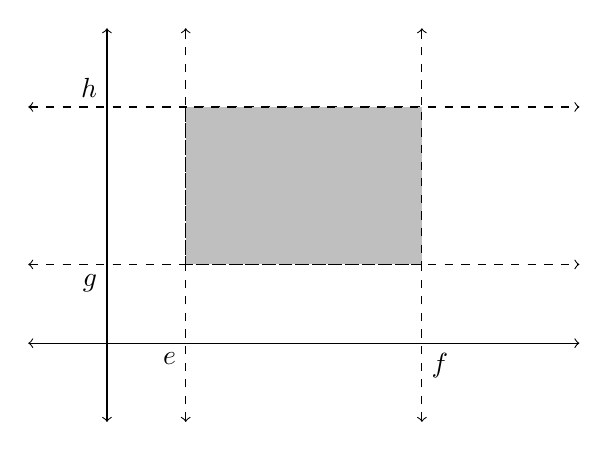
\begin{tikzpicture}
        \draw[<->] (-1,0)--(6,0);
        \draw[<->] (0,-1)--(0,4);
        \draw[<->, dashed] (-1,1)--(6,1);
        \draw[<->, dashed] (-1,3)--(6,3);
        \draw[<->, dashed] (1,-1)--(1,4);
        \draw[<->, dashed] (4,-1)--(4,4);
        \node [below left] at (1,0) {$e$};
        \node [below right] at (4,0) {$f$};
        \node [above left] at (0,3) {$h$};
        \node [below left] at (0,1) {$g$};
        \draw[dashed, fill=lightgray] (1,1) rectangle (4,3);
      \end{tikzpicture}
      \caption{Visually, we can interpret each $\mathscr{S} (U_\beta)$ as a "strip" in the total product space. For example in $\mathbb{R}^2$, there are two "strips" $(e, f) \times \mathbb{R}$ and $\mathbb{R} \times (g, h)$ that intersect. Note that each strip is the preimage of the projection mapping. }
      \label{fig:product_topology}
    \end{figure}
  \end{definition}

  We can deduce some conclusions comparing these topologies. First, the product and box topologies are precisely the same if we work in finite Cartesian products of spaces, since any element of the box topology (left hand side) can be expressed as a finite intersection of some open sets (in the right hand side). That is, if $\text{card}\,I < \infty$, then 
  \begin{equation}
    \prod_{\alpha \in I} U_i = \bigcap_{\alpha \in I} \big\{ \prod_{\gamma \in I} W_\gamma \mid W_\gamma = U_\gamma \text{ if } \gamma = \alpha, \, W_\gamma = X_\gamma \text{ if } \gamma \neq \alpha\big\}
  \end{equation}
  Secondly, we can see that the box topology is finer than the product topology (strictly finer if working in infinite product spaces). 

  \begin{example}
    The set $(0,1)^\mathbb{N} \subset \mathbb{R}^\mathbb{N}$ is clearly open in the box topology, but it is considered "too tight" to be in the product topology. However, 
    \begin{equation}
      (0,1) \times \mathbb{R} \times \mathbb{R} \times \ldots
    \end{equation}
    is open in the product topology since only one (a finite amount) of the factors is not the whole space. 
  \end{example}

  The following theorem reveals why the product topology is superior than the box topology in product spaces. 

  \begin{theorem}[Continuity of Functions Mapped to Product Topology]
    Given the function 
    \begin{equation}
      f: A \rightarrow \prod_{\alpha \in I} X_\alpha, \; f(a) \equiv \big( f_\alpha (a) \big)_{\alpha \in I}
    \end{equation}
    with its component functions $f_\alpha: A \rightarrow X_\alpha$. Let $\prod X_\alpha$ have the product topology. Then the function $f$ is continuous if and only if each function $f_\alpha$ is continuous. 
  \end{theorem}
  \begin{proof}
    We prove both directions. Let $\pi_\beta$ be the projection of this product onto the $\beta$th component space. By construction $\pi_\beta$ is continuous $\implies \pi_\beta^{-1} (U_\beta)$ is a basis element of the product topology of $\prod X_\alpha$. 
    \begin{enumerate}
      \item $(\rightarrow)$ $f$ is continuous, so $f_\beta \equiv \pi_\beta \circ f$, as the composition of continuous functions, is also continuous. 
      \item $(\leftarrow)$ Assume that each $f_\beta$ is continuous. Let there be an open set $U_\beta \subset X_\beta$. Then, the canonical open set $\pi_\beta^{-1}$ in the product space $\prod X_\alpha$ is also open. Now, the preimage of $\pi_\beta^{-1} (U_\beta)$ under $f$ is 
      \begin{align*}
        f^{-1} \big( \pi_\beta^{-1} (U_\beta)\big) & = (f^{-1} \circ \pi_\beta^{-1})(U_\beta) \\
        & = (\pi_\beta \circ f)^{-1} (U_\beta) \\
        & = f_\beta^{-1} (U_\beta)
      \end{align*}
      Since $f_\beta$ is already assumed to be continuous, $f_\beta^{-1} (U_\beta)$ is open in $A$. 
    \end{enumerate}
  \end{proof} 

  This theorem also works for the box topology only if we are working with finite product spaces. But in general, this theorem fails for the box topology. Consider the following example. 

  \begin{example}
    Let $\mathbb{R}^\omega$ be the countably infinite product of $\mathbb{R}$'s. Let us define the function 
    \begin{equation}
      f: \mathbb{R} \rightarrow \mathbb{R}^\omega
    \end{equation}
    with coordinate function defined $f_n (t) \equiv t$ for all $n \in \mathbb{N}$. Clearly, each $f_n$ is continuous. Given the box topology, we consider one basis element of $\mathbb{R}^\omega$
    \begin{equation}
      B = \prod_{i=1}^\infty (-\frac{1}{i}, \frac{1}{i})
    \end{equation}
    Assume that $f$ is continuous, that is $f^{-1}(B)$ is open in $\mathbb{R}$. Then, it would contain some finite interval $(-\delta, \delta)$ about $0$, meaning that $f\big( (-\delta, \delta)\big) \subset B$. This implies that for each $n \in \mathbb{N}$, 
    \begin{equation}
      f_n \big( (-\delta, \delta) \big) = (-\delta, \delta) \subset \Big( -\frac{1}{n}, \frac{1}{n} \Big)
    \end{equation}
    which contradicts the fact that $B$ is open, since the interval $(-1/n, 1/n)$ converges onto a point $0$. 
  \end{example}

  However, there is no useful criterion for the continuity of a mapping $f: X \times Y \longrightarrow A$ even if we have the product topology on $X \times Y$. One might conjecture that this $f$ is continuous if it is continuous in each variable separately, but this is in fact not true. 

  \begin{theorem}[Topologies on Products of Metric Spaces Coincide]
    Given a metric space
  \end{theorem}

  \begin{corollary}
    The Euclidean topology on $\mathbb{R}^n$ is equivalent to the product topology of the Euclidean topologies on $\mathbb{R}$. 
  \end{corollary} 

  \begin{theorem}[Subspace of Products and Products of Subspaces are Equivalent]
    If $A \subset X$ and $B \subset Y$, then the following topologies are equivalent. 
    \begin{enumerate}
      \item The subspace topology on the product topology of $X \times Y$. 
      \item The product topology on the subspace topologies of $A, B$. 
    \end{enumerate}
  \end{theorem}

  \begin{example}[Sorgenfrey Plane]
    The Cartesian product of two real lines with the lower limit topology is called the \textbf{Sorgenfrey plane}. 
    \begin{equation}
      \mathbb{R}_\ell \times \mathbb{R}_\ell
    \end{equation}
  \end{example}

  \begin{lemma}
    The addition, subtraction, and multiplication operations are continuous functions from $\mathbb{R} \times \mathbb{R} \longrightarrow \mathbb{R}$, and the quotient operation is a continuous function from $\mathbb{R} \times (\mathbb{R} \setminus \{0\}) \longrightarrow \mathbb{R}$. 
  \end{lemma}
  \begin{proof}
    Standard $\epsilon-\delta$ proof. 
  \end{proof}

  Now that we have defined what it means for binary operations to be continuous, we can talk about \textit{topological algebra}, which is the study of algebraic structures such that their algebraic operations and inverses are continuous. One important such concept is a \textit{topological group}, which will be mentioned later. 

\subsection{Quotient Topologies} 

  We have established natural topologies on sets that are constructed from other sets, namely by subsets and Cartesian products. Another way to construct a set is by taking an \hyperref[set-partition]{equivalence relation}, which partitions the set into its equivalence classes. The method in which we construct such a topology on this quotient space, called the \textit{quotient topology}, is slightly less straightforward.  

  \subsubsection{Quotient Maps}

    \begin{definition}[Quotient Map]
      A function $p: X \rightarrow Y$ is said to be a \textbf{quotient map} if it is surjective and 
      \begin{equation}
        U \text{ is open in } Y \iff p^{-1}(U) \text{ is open in } X
      \end{equation} 
      Note that we could have also replaced open with closed sets and the definitions are equivalent. 
    \end{definition}

    \begin{definition}[Saturation]
      A subset $S \subset X$ is \textbf{saturated} with respect to the surjective map $p: X \rightarrow Y$ if for every $p^{-1} (A)$ (where $A \subset Y$) that intersects $S$, $p^{-1}(A)$ is completely contained within $S$. That is, 
      \begin{equation}
        p^{-1} \big( p(S) \big) = S
      \end{equation}

      \begin{figure}[H]
        \centering 
        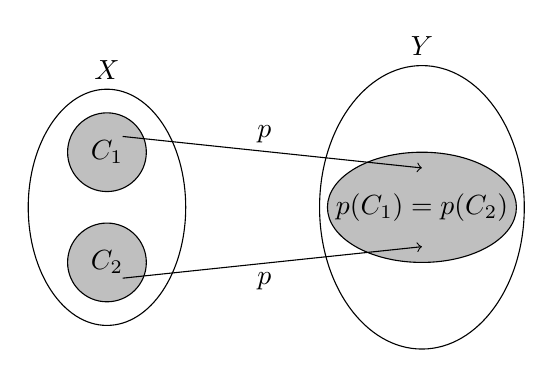
\begin{tikzpicture}
          \draw (0,0) ellipse (1 and 1.5);
          \draw[fill=lightgray] (0, 0.7) circle (0.5);
          \draw[fill=lightgray] (0, -0.7) circle (0.5);
          \node[above] at (0,1.5) {$X$};
          \draw (4,0) ellipse (1.3 and 1.8);
          \node[above] at (4,1.8) {$Y$};
          \draw[fill=lightgray] (4,0) ellipse (1.2 and 0.7);
          \node at (0, 0.7) {$C_1$};
          \node at (0,-0.7) {$C_2$};
          \node at (4,0) {$p(C_1) = p(C_2)$};
          \draw[->] (0.2,0.9)--(4,0.5);
          \draw[->] (0.2,-0.9)--(4,-0.5);
          \node[above] at (2, 0.7) {$p$};
          \node[below] at (2, -0.7) {$p$};
        \end{tikzpicture}
        \caption{We can see that $C_1$ and $C_2$ alone are not saturated, but $C_1 \cup C_2$ is saturated. Visually, for a given set $C \subset X$ to be saturated, there cannot be any points $q \not\in C$ such that $q \in p(C)$. }
        \label{fig:saturation}
      \end{figure}
    \end{definition}

    We now introduce an alternative, equivalent definition of quotient maps. 

    \begin{theorem}[Quotient Maps w.r.t. Mapping Saturated Sets]
      $p: X \rightarrow Y$ is a quotient map if and only if $p$ is continuous and $p$ maps saturated open sets of $X$ to open sets of $Y$ (or saturated closed sets of $X$ to closed sets of $Y$). 
    \end{theorem} 

    The first property is that quotient maps behave nicely under compositions. 

    \begin{theorem}[Composition of Quotient Maps]
      The composition of two quotient maps is a quotient map. 
    \end{theorem}
    \begin{proof}
      We immediately know that the composition of surjective maps are surjective and that of continuous maps are continuous. 
    \end{proof}

    However, they do not behave nicely under subspace or products. If $p: X \rightarrow Y$ is a quotient map and $A$ is a subspace of $X$, then the map $p^\prime: A \rightarrow p(A)$ obtained by restricting both the domain and codomain of $P$ need not be a quotient map. The product of two quotient maps is not necessarily a quotient map. That is, given $p: A \rightarrow B$ and $q: C \rightarrow D$ are quotient maps, the map 
    \begin{equation}
      p \times q: A \times C \rightarrow B \times D, \; (p \times q) (a \times c) \equiv p(a) \times q(c)
    \end{equation}
    is not necessarily a quotient map. 

    \begin{example}[Restriction of Quotient Maps are Not Quotient Maps]
      
    \end{example}

    \begin{example}[Products of Quotient Maps are Not Quotient Maps]
      
    \end{example}

    Additionally, quotient maps are clearly not homeomorphisms, so topological properties are not preserved. 

    \begin{example}[]
      
    \end{example}

    However, there is just one extra condition on a quotient map that will make it a homeomorphism.  

    \begin{lemma}[Bijective Quotient Maps]
      A quotient map that is injective (and hence bijective) is a homeomorphism. 
    \end{lemma} 

  \subsubsection{Open and Closed Maps}

    Open and closed functions map open/closed sets to open/closed sets, unlike continuous functions which take the preimage. However, they do are not natural and most maps are not open nor closed, so this is a pretty special condition. 

    \begin{definition}[Open, Closed Maps]
      A map $f: X \rightarrow Y$ is said to be 
      \begin{enumerate}
        \item \textbf{open} if it maps open sets of $X$ to open sets of $Y$. 
        \item \textbf{closed} if it maps open sets of $X$ to closed sets of $Y$. 
      \end{enumerate}
      Note that open and closed maps are completely independent. A map may be open, closed, neither, or both. 
    \end{definition}

    \begin{example}[Open but Not Closed]
      The projection $\pi_1: X \times Y \rightarrow X$ is an open map but but closed. Consider $\pi_1: \mathbb{R}^2 \rightarrow \mathbb{R}$ with $S = \{(x, y) \in \mathbb{R}^2 \mid xy = 1 \}$. Then $\pi_1 (S) = \mathbb{R} \setminus \{0\}$, which is not closed.\footnote{In open maps, the typical behavior is that points are ``copied,'' i.e. for projections, the preimage of $\pi_1^{-1} (x) = x \times Y$, where all $y \in Y$ are copied.}
    \end{example}

    \begin{example}[Closed but Not Open]
      $f: \mathbb{R} \rightarrow \mathbb{R}$ with $f(x) = x^2$ is closed but not open since $f(\mathbb{R}) = [0, +\infty)$ which is not open. 
    \end{example}

    Note that an open map or a closed map (with continuous and surjective) are trivially quotient maps. Since given a $U \subset Y$ with $f^{-1} (U)$ open, then by definition $U = f(f^{-1} (U))$ is open by definition. 

    \begin{theorem}[Open/Closed Maps are Stronger than Quotient Maps]
      If $p: X \rightarrow Y$ is a surjective, continuous map that is either open or closed (that is, maps open sets to open sets or closed sets to closed sets), then $p$ is a quotient map.\footnote{Note however, that the converse is not true; there exists quotient maps that are neither open nor closed. }
    \end{theorem} 

    \begin{example}[Quotient Maps that are Neither Open Nor Closed]
      
    \end{example}

  \subsubsection{Quotient Topology}

    Now that we have defined the quotient map, we are ready to define the quotient topology. 

    \begin{definition}[Quotient Topology]
      Let $p: (X, \T_X) \rightarrow Y$ be a surjective map.\footnote{A natural surjective map that we can construct is by taking an equivalence relation $\sim$ on $X$, setting $Y = X/{\sim}$, and taking $p: x \mapsto [x]$. Every surjective map can be thought of as a map induced by an equivalence relation, since we can set $x \sim x^\prime$ iff $f(x) = f(x^\prime)$, so these are equivalent.} Then, the \textbf{quotient topology} induced by $p$ is defined in the following equivalent ways. 
      \begin{enumerate}
        \item It is the final topology on the quotient set $X/{\sim}$ wrt the projection map $p$. 
        \item It is the topology of all subsets $U$ of $Y$ s.t. $p^{-1}$ is open in $X$. 
        \begin{equation}
          U \text{ open in } X/{\sim} \iff p^{-1} (U) \text{ saturated and open in } X
        \end{equation}
        \item It is the unique topology $\T_Y$ relative to which $p$ is a quotient map.\footnote{We claim that this topology exists and is unique.}
      \end{enumerate}
      The quotient set $X/{\sim}$ with its quotient topology is called the \textbf{quotient space}. 
    \end{definition}
    \begin{proof}
      The topology $\T_Y$ on $Y$ is defined by letting it consist of all subsets $U$ of $Y$ such that $p^{-1}(U)$ is open in $X$. This is indeed a topology since
      \begin{enumerate}
        \item $p^{-1} (\emptyset) = \emptyset$ and $p^{-1}(Y) = X$
        \item $p^{-1} \Big( \bigcup_{\alpha \in J} U_\alpha \Big) = \bigcup_{\alpha \in J} p^{-1} (U_\alpha)$
        \item $p^{-1} \Big( \bigcap_{i=1}^n U_i \Big) = \bigcap_{i=1}^n p^{-1} (U_i)$
      \end{enumerate}
    \end{proof}

    The intuition is the following. The topology on $X$ is fixed, and we must somehow find some topology on $Y$ that makes $p$ a quotient map. If we make $\T_Y$ too coarse, satisfiying continuity of $p$ is easy but it may not necessarily mean that $p^{-1}(U)$ open in $X$ implies $U$ open in $Y$. However, if we make $\T_Y$ too fine, then continuity may not be satisifed. The theorem states that there is a middle point---in fact exactly one topology---in which cases both directions are satisfied. 

    \begin{example}
      Let $p: (\mathbb{R}, \T_\mathbb{R}) \rightarrow \mathbb{R} / 2 \pi \mathbb{R}$. Then, the final topology of $\mathbb{R} / 2 \pi \mathbb{R}$ would be simply defined 
      \begin{equation}
        \T_{\mathbb{R} / 2 \pi \mathbb{R}} \equiv \{U \subset \mathbb{R} / 2\pi \mathbb{R} \mid U = p(O), O \in \T_\mathbb{R}\}
      \end{equation}
      That is, the quotient topology is merely the set of all images of open sets in $\mathbb{R}$ under $f$. However, if $\mathbb{R} / 2 \pi \mathbb{R}$ has the discrete topology $2^X$, then a single equivalence class, say $[0]$, will get mapped to the collection of points $\{2 \pi k \mid k \in \mathbb{Z}\}$, which is clearly not open in $\mathbb{R}$. Note that the final topology (or the quotient topology) is endowed onto the codomain in order to make $f$ continuous (or a quotient mapping). 
    \end{example}

    \begin{example}
      Let $X \equiv [0,1] \cap [2,3] \subset \mathbb{R}$ and $Y y \equiv [0,2] \subset \mathbb{R}$. Then, we define $p: X \rightarrow Y$ as 
      \begin{equation}
        p(x) \equiv \begin{cases} x & x \in [0,1] \\ x-1 & x \in [2,3] \end{cases}
      \end{equation}
      $p$ is continuous (under subspace topology of $X \subset \mathbb{R}$), surjective, and closed, meaning that it is a quotient map. However, it is not open, since the image of the open set $[0,1]$ of $X$ is $[0,1]$, which is not open in $Y$. 
    \end{example}

    \begin{example}[Finite Sets]
      Let $p: \mathbb{R} \rightarrow \{a, b, c\}$ be defined as 
      \begin{equation}
        p(x) \equiv \begin{cases} a & x > 0 \\ b & x < 0 \\ c & x = 0 \end{cases}
      \end{equation}
      Then, the quotient topology of $\{a, b, c\}$ consists of 
      \begin{equation}
        \emptyset, \{a\}, \{b\}, \{a, b\}, \{a, b, c\}
      \end{equation}
    \end{example}

    Okay, so we've learned yet another way to construct topologies. However, things become interesting when we start to compare quotient spaces to other topological spaces that we already know of. The following series of theorems will help in our analysis. 

    \begin{theorem}[Induced Maps from Quotient Space]
      Let $p: X \rightarrow Y$ be a quotient map (e.g. $Y = X/{\sim}$ for some ER $\sim$). Let $f: X \rightarrow Z$ be a function such that if $p(x) = p(x^\prime)$, then $f(x) = f(x^\prime)$, i.e. $x \sim x^\prime \iff f(x) = f(x^\prime)$. Then, 
      \begin{enumerate}
        \item $f$ induces the map $\bar{f}$ satisfying $f = \bar{f} \circ p$. 

        \begin{figure}[H]
          \centering 
          \begin{tikzcd}
            X \arrow{d}{p} \arrow{r}{f} & Z\\
            X/{\sim} \arrow{ru}{\bar{f}} & 
          \end{tikzcd}
          \caption{The theorem states that the diagram commutes. } 
          \label{fig:quotient_continuity}
        \end{figure}

        \item $f$ continuous iff $\bar{f}$ continuous. 
        \item $f$ quotient map iff $\bar{f}$ quotient map. 
      \end{enumerate}
    \end{theorem}
    \begin{proof}
      Listed. 
      \begin{enumerate}
        \item 
        \item Suppose $f$ is continuous. Let $U \subset Z$ be open. Then we need to show that $\bar{f}^{-1} (U)$ is open. But we can see that $p^{-1} (\bar{f}^{-1}(U)) = f^{-1} (U)$ is open since $f$ is continuious. Therefore $\bar{f}^{-1} (U)$ is open since $p$ is a QM.If $\bar{f}$ is continuous, then $f = \bar{f} \circ p$ is continuous as the composition of continuous maps. 
        \item Suppose $f$ is a quotient map with $U \subset Z$ s.t. $\bar{f}^{-1} (U)$ is open. We need to show that $U$ is open. Then $p^{-1} (\bar{f}^{-1} (U))$ is open since $p$ is continuous $\implies f^{-1} (U)$ is open. But $f$ is a quotient map, so $U$ is open. 
      \end{enumerate}
    \end{proof}

    \begin{corollary}
      If $f$ is a quotient map, then $\bar{f}$ is a homeomorphism. 
    \end{corollary}
    \begin{proof}
      Show that $\bar{f}$ is injective, and so its bijective. Since it's a quotient map, it's a homeomorphism. 
    \end{proof}

    Therefore we can just make up any equivalence relation (surjective map) on $X$ which gives us a quotient space $X/{\sim}$. To figure out whether this quotient space is homeomorphic to a topological space that we already know, we first (cleverly) choose a candidate space $Z$ and try to write a quotient map $f: X \rightarrow Z$ that ``agrees'' with the equivalence relation, i.e. $x \sim x^\prime \iff f(x) = f(x^\prime)$. We don't need to worry too much about surjectivity, since if we have continuity and the ``reverse continuity'' conditions satisfied then we can just restrict $Z$ to the image of $f$ to make it surjective anyways. Once we have found such a quotient map $f$, using the theorem above we can conclude that $X/{\sim}$ is homeomorphic to $Z$, and we are done! We show various examples in the next section. 

    We end this section with a warning. It was the case that a lot of the properties get passed down to subspaces, but this is not the case for quotient maps. 

    \begin{example}[Quotient Topology Reduced to Trivial Topology]
      \label{quotient_trivial}
      Let $X = \mathbb{R}$ with $x \sim y \iff x - y \in \mathbb{Q}$. We claim that $X/{\sim}$ is uncountable. If we wish to find open sets in $X/{\sim}$, we can do this by finding saturated open sets in $X$. Let $U \subset \mathbb{R}$ be open and saturated. Since it is open, by the density of $\mathbb{Q}$ in $\mathbb{R}$, $U$ must contain a rational number $\implies \mathbb{Q} \subset U$, and so $U = \mathbb{R}$. Therefore the only saturated open sets are $\emptyset, \mathbb{R}$, meaning that $X/{\sim}$ has the trivial topology. 
    \end{example}

    This has a lot of consequences, and even very mild topological properties can be broken in quotient spaces.  

    \begin{example}[Quotient of Hausdorff Space Need not be Hausdorff]
      \label{quotient_hausdorff}
      Given $X = \mathbb{R}^2 \setminus \{0\}$ with the ER defined $(x, y) \sim (x^\prime, y^\prime)$ iff $x = x^\prime$, and if $x = x^\prime = 0$, then $\mathrm{sign}(y) = \mathrm{sign}(y^\prime)$. This is the line with 2 origins with the quotient map 
      \begin{equation}
        f(x, y) = \begin{cases} 
          x \text{ if } x \neq 0 \\
          a \text{ if } x = 0, y > 0 \\ 
          b \text{ if } x = 0, y < 0
        \end{cases}
      \end{equation}
    \end{example}

  \subsubsection{Quotient Spaces}

    \begin{example}[1-Sphere]
      Let $X = [0, 1]$ with $\sim$ defined only with $0 \sim 1$. Then our intuition may tell us that by ``sticking'' the endpoints together, we can get a unit circle $S^1$. 

      \begin{figure}[H]
        \centering
        \begin{subfigure}[b]{0.48\textwidth}
          \centering
          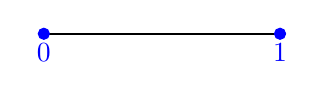
\begin{tikzpicture}
            % Draw the line segment from 0 to 1
            \draw[thick] (0,0) -- (3,0);
            
            % Draw blue endpoints
            \filldraw[blue] (0,0) circle (2pt) node[below] {0};
            \filldraw[blue] (3,0) circle (2pt) node[below] {1};
          \end{tikzpicture}
          \caption{Unit interval $[0, 1]$}
          \label{fig:unit-interval}
        \end{subfigure}
        \hfill 
        \begin{subfigure}[b]{0.48\textwidth}
          \centering
          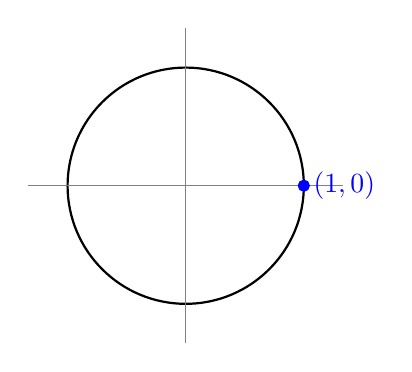
\begin{tikzpicture}
            % Draw the unit circle
            \draw[thick] (0,0) circle (1.5);
            
            % Draw axes for reference
            \draw[gray, thin] (-2,0) -- (2,0);
            \draw[gray, thin] (0,-2) -- (0,2);
            
            % Mark the point (1,0) in blue
            \filldraw[blue] (1.5,0) circle (2pt) node[right] {$(1,0)$};
          \end{tikzpicture}
          \caption{Unit circle $S^1$ in $\mathbb{R}^2$}
          \label{fig:unit-circle}
        \end{subfigure}
        \caption{Visual of the homeomorphism between $[0, 1]$ and $S^1$.}
        \label{fig:comparison}
      \end{figure}

      So can I come up with a function $f: [0, 1] \rightarrow S^1$ s.t. $f(0) = f(1)$? Yes, we can define 
      \begin{equation}
        \bar{f}(x) = (\cos{2 \pi x}, \sin{2\pi x})
      \end{equation} 
      which indeed satisfies $f(0) = f(1) \iff 0 \sim 1$.\footnote{Note that we could just chosen $\mathbb{R}^2$ and restricted the image to $S^1$ at the end as well.} Therefore, by the theorem above, $X/{\sim} \cong S^1$, defined by the homeomorphism $\bar{f}(x) = (\cos{2 \pi x}, \sin{2\pi x})$.  
    \end{example}

    \begin{example}[Alternative Construction of 1-Sphere]
      Let $X = \mathbb{R}$ with $\sim$ defined $x \sim y$ iff $x - y \in \mathbb{Z}$. We call this $\mathbb{R}/\mathbb{Z}$. Our intution tells us that by ``folding'' the real number line into overlapping unit intervals, we can get the unit circle. We will show that
      \begin{equation}
        \frac{\mathbb{R}}{\mathbb{Z}} \cong S^1
      \end{equation}
      Let us construct the set $(\mathbb{R}, \T_{\mathbb{R}})$ with paramater $t$. We define maps
      \begin{align*}
        p: \mathbb{R} \rightarrow \mathbb{R} / \mathbb{Z}, \;\; p(t) \equiv t \; (\text{mod } 1) \\
        q: \mathbb[R] \rightarrow S^1 \subset \mathbb{C}, \;\; g(t) \equiv e^{2 \pi i t} 
      \end{align*}
      We claim that $p$ and $q$ are both quotient mappings. Clearly, $p$ is a quotient mapping. As for $q$, it it easy to see that it is surjective (but not injective) and continuous ($\T_{S^1}$ has the basis of open intervals on $S^1$). It is also easy to notice that given an open interval $U \subset S^1$, $q^{-1}(U)$ will be the union of open intervals equally spaced in $\mathbb{R}$. Additionally, given any open interval in $\mathbb{R}$, it maps to an open interval in $S^1$ (note that $S^1$ itself is also open). These three conditions imply that $q$ is a quotient map. We now define maps 
      \begin{align}
        q \circ p^{-1}: & \mathbb{R} / \mathbb{Z} \rightarrow S^1 \\
        p \circ q^{-1}: & S^1 \rightarrow \mathbb{R} / \mathbb{Z}
      \end{align}
      and claim that these maps are homeomorphisms. We can clearly see that the mapping from an open set in $\mathbb{R} / \mathbb{Z}$ to the union of spaced open intervals in $\mathbb{R}$ is an injection, and the mapping from this union of open intervals to the union of open intervals in $S^1$ is a surjection. The composition of these two mappings clearly defines a bijection. Therefore, $q \circ p^{-1}$ is proven to be a bicontinuous bijective mapping between open sets $U \subset \mathbb{R} / \mathbb{Z}$ and $V \subset S^1 \implies$ $q \circ p^{-1}$ is a homeomorphism. 

      This result clearly makes sense since 
      \begin{equation}
        \frac{\mathbb{R}}{\mathbb{Z}} \cong \frac{[0,1]}{\sim}
      \end{equation}
      where the relation $\sim$ maps every point $x \in (0,1)$ to its own equivalence class and the points $0, 1$ to one equivalence class $\{0\}$. Therefore, it is informally said that the quotient space of the real line is a circle. 

      One may attempt to construct a simpler set by replacing $S^1$ with the half-open interval $[0,1)$. However, while $[0,1)$ is bijective to $\mathbb{R} / \mathbb{Z}$,
      \begin{equation}
        \frac{\mathbb{R}}{\mathbb{Z}} \not\cong [0,1)
      \end{equation}
      That is, the two sets are not homeomorphic because the topologies of $[0,1)$ and $\mathbb{R} / \mathbb{Z}$ are not compatible. For instance, when we attempt to map the open set 
      \begin{equation}
        \bigg\{ [x] \in \mathbb{R} / \mathbb{Z} \mid 0 \leq x \leq \frac{1}{4} \vee x > \frac{1}{2} \bigg\} \in \T_{\mathbb{R} / \mathbb{Z}}
      \end{equation}
      to $\T_{[0,1)}$, it does not return an open set. 

      Furthermore, this means that
      \begin{equation}
        S^1 \times S^1 \cong \frac{[0,1]^2}{\sim^\prime} \cong \bigg( \frac{\mathbb{R}}{\mathbb{Z}} \bigg)^2
      \end{equation}
      where $\sim^\prime$ is the quotient mapping defined in the previous construction of the torus. 
    \end{example}

    \begin{example}[Annulus]
      Let $X = [0, 1]^2$ with $\sim$ defined $(0, y) \sim (1, y)$ for all $y \in [0, 1]$. Then our intuition may tell us that by sticking the top and bottom together, we can get an annulus, defined as the closed region $A \subset \mathbb{R}^2$ between the disk of radius 2 and disk of radius 1. 

      \begin{figure}[H]
        \centering
        \begin{subfigure}[b]{0.48\textwidth}
          \centering
          \begin{tikzpicture}
            % Draw square
            \draw (0,0) rectangle (2,2);
            
            % Label right and left with > rotated to point up
            \node at (2,1) {$\rotatebox{90}{>}$};
            \node at (0,1) {$\rotatebox{90}{>}$};
          \end{tikzpicture}
          \caption{Unit square $[0,1] \times [0,1]$}
          \label{fig:unit-square}
        \end{subfigure}
        \hfill 
        \begin{subfigure}[b]{0.48\textwidth}
          \centering
          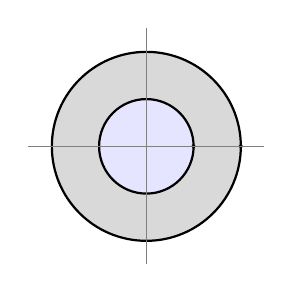
\begin{tikzpicture}[scale=0.6]
            % Fill the annular region with grey (using even-odd rule to keep the inner circle empty)
            \begin{scope}
              \clip (0,0) circle (2);
              \fill[gray!30] (0,0) circle (2);
              \fill[blue!10] (0,0) circle (1);
            \end{scope}
            
            % Draw the two circles
            \draw[thick] (0,0) circle (1);   % Unit circle
            \draw[thick] (0,0) circle (2);   % Circle of radius 2
            
            % Label only the points (1,0) and (2,0)
            \filldraw[font=\footnotesize] (1,0) circle (1pt) node[below] {};
            \filldraw[font=\footnotesize] (2,0) circle (1pt) node[below] {};

            \draw[gray, thin] (-2.5,0) -- (2.5,0);
            \draw[gray, thin] (0,-2.5) -- (0,2.5);
          \end{tikzpicture}
          \caption{Annular region between circles of radius 1 and 2}
          \label{fig:annular-region}
        \end{subfigure}
        \caption{Unit square and annular region}
        \label{fig:annular_comparison}
      \end{figure} 

      We can indeed come up with the function $f:[0, 1]^2 \rightarrow A$ defined 
      \begin{equation}
        (x, y) \mapsto \big( (1 + y) \cos{2 \pi x}, (1 + y) \sin{2 \pi x} \big) \in \mathbb{R}^2
      \end{equation}
      which satisfies $(0, y) \sim (1, y) \iff f(0, y) = f(1, y)$. Therefore by the theorem above $X/{\sim} \cong A$. 
    \end{example}

    \begin{example}[Cylinder]
      Let $X = [0, 1]^2$ with $\sim$ defined $(0, y) \sim (1, y)$ for $y \in [0, 1]$. Then our intuition may tell us that by sticking the top and bottom together, we can get the cylinder, defined as $C \equiv \{(x, y, z) \in \mathbb{R}^3 \mid x^2 + y^2 = 1, z \in [0,1]\}$.

      \begin{figure}[H]
        \centering
        \begin{subfigure}[b]{0.48\textwidth}
          \centering
          \begin{tikzpicture}
            % Draw square
            \draw (0,0) rectangle (2,2);
            
            % Label right and left with > rotated to point up
            \node at (2,1) {$\rotatebox{90}{>}$};
            \node at (0,1) {$\rotatebox{90}{>}$};
          \end{tikzpicture}
          \caption{Cylinder as an equivalence class on $[0, 1]^2$.}
          \label{fig:cylinder_equiv}
        \end{subfigure}
        \hfill 
        \begin{subfigure}[b]{0.48\textwidth}
          \centering
          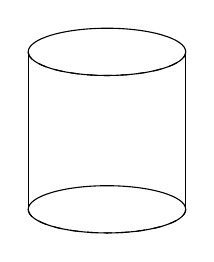
\begin{tikzpicture}
            % Draw cylinder
            \draw (0,0) ellipse (1 and 0.3);
            \draw (0,2) ellipse (1 and 0.3);
            \draw (-1,0) -- (-1,2);
            \draw (1,0) -- (1,2);
            
            % Draw dashed lines to show back of cylinder
            \draw[dashed] (-1,0) arc (180:360:1 and 0.3);
            \draw[dashed] (-1,2) arc (180:360:1 and 0.3);
          \end{tikzpicture}
          \caption{Cylinder as an embedding in $\mathbb{R}^3$. }
          \label{fig:cylinder_embed}
        \end{subfigure}
        \caption{Two geometric figures: a square with labeled sides and a cylinder}
        \label{fig:cylinder}
      \end{figure}
      
      We can indeed come up with the function $f: [0, 1]^2 \rightarrow C$, defined
      \begin{equation}
        (x, y) \mapsto \big( \cos{2\pi x}, \sin{2 \pi x}, y \big)
      \end{equation}
      which satisfies $(0, y) \sim (1, y) \iff f(0, y) = f(1, y)$. Therefore by the theorem above $X/{\sim} \cong C$. 
    \end{example}

    \begin{example}[Torus]
      Let $X = [0,1]^2$ with $\sim$ defined $(0, y) \sim (1, y)$ for $y \in [0, 1]$ and $(x, 0) \sim (x, 1)$ for $x \in [0, 1]$. Then our intuition may tell us that by first sticking the sides together, we get a cylinder, and by sticking the top with the bottom, we get a torus, denoted $T^2$. 

      \begin{figure}[H]
        \centering
        \begin{subfigure}[b]{0.48\textwidth}
          \centering
          \begin{tikzpicture}
            % Draw square
            \draw (0,0) rectangle (2,2);
            
            % Label top and bottom with >
            \node at (1,2) {$>$};
            \node at (1,0) {$>$};
            
            % Add >> labels to left and right sides, rotated to point upward
            \node[rotate=90] at (0,1) {$>>$};
            \node[rotate=90] at (2,1) {$>>$};
          \end{tikzpicture}
          \caption{Torus as an equivalence class on $[0, 1]^2$.}
          \label{fig:square_torus}
        \end{subfigure}
        \hfill 
        \begin{subfigure}[b]{0.48\textwidth}
          \centering
          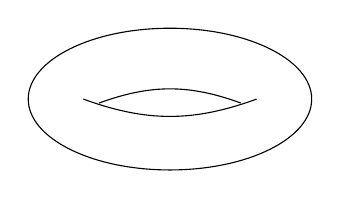
\begin{tikzpicture}
            % Draw torus similar to the reference image
            % Outer ellipse (complete)
            \draw (0,0) ellipse (1.8 and 0.9);
            
            % Inner curves (representing the hole)
            \draw (-0.9, -0.05) to[out=20,in=-200] (0.9, -0.05);
            \draw (-1.1, 0) to[out=-20,in=200] (1.1, 0);
          \end{tikzpicture}
          \caption{Torus as an embedding in $\mathbb{R}^3$.}
          \label{fig:torus}
        \end{subfigure}
        \caption{Representations of a torus.}
        \label{fig:geometric-figures}
      \end{figure}

      We can indeed come up with a function $f: [0, 1]^2 \rightarrow T^2 \subset \mathbb{R}^3$. 
      \begin{equation}
        (x, y) \mapsto \big( (2 + \cos{2 \pi x}) \cos{2\pi y}, (2 + \cos{2 \pi x}) \sin{2 \pi y}, \sin{2 \pi x} \big)
      \end{equation}
      which is consistent with the relation.  

      \begin{figure}[H]
        \centering 
        \begin{tikzpicture}
          \draw (0,0) rectangle (2,2);
          \draw (3,0) rectangle (5,2);
          \draw (6,0) rectangle (8,2);
          \draw (9,0) rectangle (11,2);
          \draw[dashed] (1, 1.5) circle [radius=0.4];
          \draw[fill] (1, 1.5) circle [radius=0.03];
          \draw[dashed] (3.9,0) arc (0:180: 0.4);
          \draw[dashed] (3.9,2) arc (0:-180:0.4);
          \draw[dashed] (6,1.1) arc (-90:90:0.4);
          \draw[dashed] (8,1.9) arc (90:270:0.4);
          \draw[fill] (3.5,0) circle [radius=0.03];
          \draw[fill] (3.5,2) circle [radius=0.03];
          \draw[fill] (6,1.5) circle [radius=0.03];
          \draw[fill] (8,1.5) circle [radius=0.03];
          \draw[fill] (9,0) circle [radius=0.03];
          \draw[fill] (11,0) circle [radius=0.03];
          \draw[fill] (9,2) circle [radius=0.03];
          \draw[fill] (11,2) circle [radius=0.03];
          \draw[dashed] (9.4,0) arc (0:90:0.4);
          \draw[dashed] (9.4,2) arc (0:-90:0.4);
          \draw[dashed] (11,0.4) arc (90:180:0.4);
          \draw[dashed] (10.6,2) arc (180:270:0.4);
        \end{tikzpicture}
        \caption{The quotient topology of this quotient space consists of open sets of form. } 
        \label{fig:torus_basis}
      \end{figure}
      We can check that this mapping is indeed a quotient map. First, it is clearly surjective. By realizing that individual points on the edge of $[0,1]^2$ are open sets themselves (by the subspace topology), we can prove that this map is indeed open and continuous. Therefore, we can see that the induced map $\hat{f}: [0, 1]^2/{\sim} \rightarrow T^2$ is a homeomorphism. 
    \end{example}

    \begin{example}[Mobius Strip] 
      Let $X = [0, 1]^2$ with $\sim$ defined $(x, 0) \sim (1-x, 1)$ for $x \in [0, 1]$. Then our intuition may tell us that by flipping over the square and sticking the sides together, we get a weird strip, called the \textbf{Mobius strip} and denoted $M_1$.  

      \begin{figure}[H]
        \centering
        \begin{subfigure}[b]{0.48\textwidth}
          \centering
          \begin{tikzpicture}
            % Draw square
            \draw (0,0) rectangle (2,2);
            
            % Label top and bottom with >
            \node at (1,2) {$>$};
            \node at (1,-0) {$<$};
          \end{tikzpicture}
          \caption{Cylinder as an equivalence class on $[0, 1]^2$.}
          \label{fig:mobius_equiv}
        \end{subfigure}
        \hfill 
        \begin{subfigure}[b]{0.48\textwidth}
          \centering 
          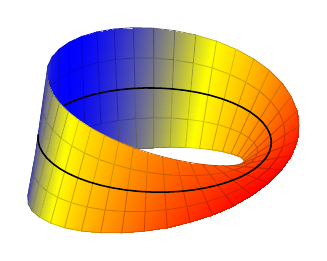
\begin{tikzpicture}[scale=0.7]
            \begin{axis}[
                hide axis,
                view={40}{40}
            ]
            \addplot3 [
                surf, shader=faceted interp,
                point meta=x,
                samples=40,
                samples y=5,
                z buffer=sort,
                domain=0:360,
                y domain=-0.5:0.5
            ] (
                {(1+0.5*y*cos(x/2)))*cos(x)},
                {(1+0.5*y*cos(x/2)))*sin(x)},
                {0.5*y*sin(x/2)});

            \addplot3 [
                samples=50,
                domain=-145:180, % The domain needs to be adjusted manually, depending on the camera angle, unfortunately
                samples y=0,
                thick
            ] (
                {cos(x)},
                {sin(x)},
                {0});
            \end{axis}
          \end{tikzpicture} 
          \caption{Mobius strip has 1 side and is a non-orientable surface.} 
          \label{fig:mobius_strip_r3}
        \end{subfigure}
        \caption{Two geometric figures: a square with labeled sides and a cylinder}
        \label{fig:mobius_strip}
      \end{figure}

      We can indeed come up with a function $f: [0, 1]^2 \rightarrow M_1 \subset \mathbb{R}^3$ 
      \begin{equation}
        (x, y) = \bigg( \cos{y} \Big[ 1 + \frac{x}{2} \cos{\frac{y}{2}} \Big], \sin{y} \Big[ 1 + \frac{x}{2} \cos{\frac{y}{2}} \Big], \frac{x}{2} \sin \frac{y}{2} \bigg)
      \end{equation}
    \end{example}

    \begin{example}[Klein Bottle]
      Let $X = [0, 1]^2$ with $\sim$ defined $(0, y) \sim (1, y)$ for $y \in [0, 1]$ and $(x, 0) \sim (1 - x, 1)$ for $x \in [0, 1]$. We cannot actually visualize this in $\mathbb{R}^3$, but we may try to construct the cylinder by sticking the left/right sides together, and then trying to glue the top and bottom in opposite direction, which gives us a \textbf{Klein Bottle}, denoted $K^2$. 

      \begin{figure}[H]
        \centering
        \begin{subfigure}[b]{0.48\textwidth}
          \centering
          \begin{tikzpicture}
            % Draw square
            \draw (0,0) rectangle (2,2);
            
            % Label top and bottom with >
            \node at (1,2) {$<$};
            \node at (1,0) {$>$};
            
            % Add >> labels to left and right sides, rotated to point upward
            \node[rotate=90] at (0,1) {$>>$};
            \node[rotate=90] at (2,1) {$>>$};
          \end{tikzpicture}
          \caption{Klein bottle as an equivalence class on $[0, 1]^2$.}
          \label{fig:square_klein}
        \end{subfigure}
        \hfill 
        \begin{subfigure}[b]{0.48\textwidth}
          \centering
          \begin{tikzpicture}[scale=0.3]
            \coordinate (P1) at (4.9,6.7);
            \coordinate (P2) at (2.5,5.4);
            \coordinate (P3) at (1.6,4);
            \Coordinate{e5b}{3.6,1.3}
            \Coordinate{e4l}{0.7,4.8}
            \Coordinate{e4r}{9.9,3.7}
            \Coordinate{si}{4.5,7.4}
            \Coordinate{bottom}{6.8,0.9}
            {[thin,black] % Changed from very thick to thin
              \draw (e4l) to[out=270,in=160,looseness=1] (P3);
              \draw (P3) to[out=340,in=270,looseness=0.3] node[above,pos=0.7,black] {} (e4r);
              \draw[name path=P2e4r] (P2) to[out=120,in=80,looseness=3.7] node[below left,pos=0.7,black] {} (e4r);
              \draw[name path=P1P1] (P1) to[out=160,in=270,looseness=1] (2.6,9) to[out=90,in=90,looseness=1.3] node[above, pos=0.5,black] {} (6.6,9.6) to[out=270,in=40,looseness=1]  (P1) ;
              \draw (P2) to[out=315,in=315,looseness=0.5] node[below right,pos=0.5,black] {} (P1);
              \draw[dashed] (P2) to[out=135,in=135,looseness=0.5] node[below right,pos=0.5,black] {} (P1);
              \draw (P2) to[out=220,in=90,looseness=1] (P3);
              \draw (P3) to[out=270,in=150,looseness=1] (e5b);
              \draw (e4l) to[out=270,in=160,looseness=1.3] (e5b);
              \draw (e5b) to[out=340,in=260,looseness=1.1] (e4r);
              \draw[dashed] (P2) to[out=300,in=330,looseness=1] (e5b);
              \draw[dashed] (e4l) to[out=90,in=90,looseness=0.6] (e4r);
              \draw[dashed] (P1) to[out=320,in=190,looseness=0.4] (bottom);
              \draw (P1) to[out=110,in=300,looseness=1] (si);
              \draw (si) to[out=120,in=270,looseness=1] (4,8.5) to[out=90,in=180,looseness=1] (5.2,9.7) to[out=0,in=90,looseness=1] (6,9) to[out=270,in=20,looseness=1] (si);
              \path[name path=e4lsi] (e4l) to[out=90,in=200,looseness=0.8] (si);
              \draw[name intersections={of=e4lsi and P2e4r}] (e4l) to[out=90,in=210,looseness=1] (intersection-1) coordinate (h1);
              \draw[dashed] (intersection-1) to[out=30,in=200,looseness=0.6] (si);
            }
          \end{tikzpicture}
          \caption{Klein bottle cannot be visualized in $\mathbb{R}^3$. Credits \href{https://tex.stackexchange.com/questions/77606/making-a-labeled-klein-bottle-using-tikz-or-pgfplots}{here}.}
          \label{fig:klein_r3}
        \end{subfigure}
        \caption{Representations of a torus. Note that we can write a continuous function from $K^2$ to $\mathbb{R}^3$, but it is not injective and therefore not a homeomorphism, which is why there is a self-intersection. }
        \label{fig:klein}
      \end{figure}

      We just claim that there exists a function $f: [0, 1]^2 \rightarrow K^2 \subset \mathbb{R}^4$.\footnote{However, an embedding in $\mathbb{R}^3$ is not possible. We will need algebraic topology to prove this.} 
    \end{example}

    \begin{example}[2-Sphere]
      Let $X$ be the closed unit disk $\{(x, y) \in \mathbb{R}^2 \mid x^2 + y^2 \leq 1\} \subset \mathbb{R}^2$ with $\sim$ defined as $x \sim y \iff x, y \in S^1$. Then our intuition may tell us that by squishing the edges of the disk into a point, we can construct a \textbf{2-sphere}, denoted $S^2 \coloneqq \{(x, y, z) \in \mathbb{R}^3 \mid x^2 + y^2 + z^2 = 1\}$. 

      \begin{figure}[H]
        \centering
        \begin{subfigure}[b]{0.48\textwidth}
          \centering
          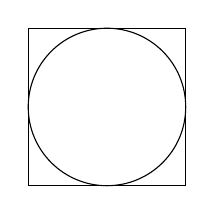
\begin{tikzpicture}
            \draw (0,0) rectangle (2,2);
            \draw (1,1) circle [radius=1];
          \end{tikzpicture}
          \caption{2-sphere as an equivalence class on the unit disk which is homeomorphic to the unit square.}
          \label{fig:S2_disk}
        \end{subfigure}
        \hfill 
        \begin{subfigure}[b]{0.48\textwidth}
          \centering
          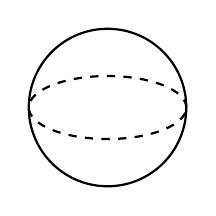
\begin{tikzpicture}
            \def\R{1}   % Radius
            \draw[thick] (0,0) circle (\R);
            \draw[thick, dashed] (0,0) ellipse ({\R} and {0.4*\R});
          \end{tikzpicture}
          \caption{2-sphere as an embedding in $\mathbb{R}^3$.}
          \label{fig:S2_R3}
        \end{subfigure}
        \caption{Representation of a sphere.}
        \label{fig:2sphere}
      \end{figure}

      We can indeed come up with a function $f: [0,1]^2 \rightarrow S^2$, defined 
      \begin{equation}
        (x, y) \mapsto \big( \sin{x} \cos{y}, \sin{x} \sin{y}, \cos{x} \big)
      \end{equation}

      \begin{figure}[H]
        \centering 
        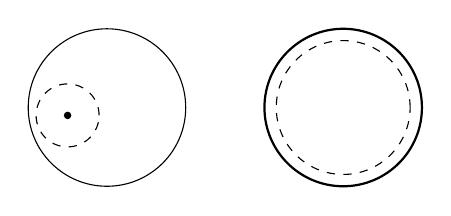
\begin{tikzpicture}
          \draw (1,1) circle [radius=1];
          \draw[thick] (4,1) circle [radius=1];
          \draw[dashed] (0.5,0.9) circle [radius=0.4];
          \draw[fill] (0.5,0.9) circle [radius=0.04];
          \draw[dashed] (4,1) circle [radius=0.85];
        \end{tikzpicture}
        \caption{The saturated open sets of $X$ consist of open sets of one of the two forms. } 
        \label{fig:open_in_s2}
      \end{figure}
    \end{example} 

    \begin{example}[Weird Quotient Space]
      Given $(\mathbb{R}, \T_{\mathbb{R}})$, let us define the relation $\sim$ determined by the quotient mapping 
      \begin{equation}
        p(x) \equiv \begin{cases} \{x\} & x \not\in \mathbb{Z} \\ \mathbb{Z} & x \in \mathbb{Z} \end{cases}
      \end{equation}
      In words, this quotient map maps every integer to the equivalence class $[0]$ and maps every other point to its own class. 

      \begin{figure}[H]
        \centering 
        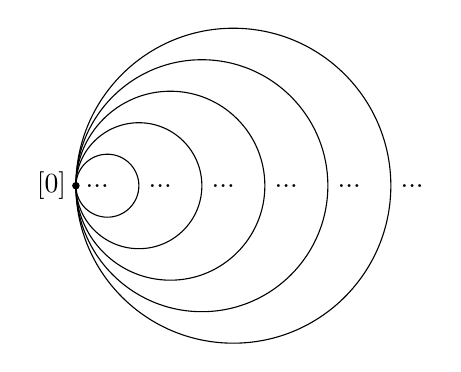
\begin{tikzpicture}[scale=0.4]
          \draw (5,0) circle (5);
          \node[left] at (0,0) {$[0]$};
          \draw[fill] (0,0) circle (0.1);
          \draw (4,0) circle (4);
          \draw (3,0) circle (3);
          \draw (2,0) circle (2);
          \draw (1,0) circle (1);
          \node[right] at (0,0) {...};
          \node[right] at (2,0) {...};
          \node[right] at (4,0) {...};
          \node[right] at (6,0) {...};
          \node[right] at (8,0) {...};
          \node[right] at (10,0) {...};
        \end{tikzpicture}
        \caption{It turns out that every interval $[j, j+1] \subset \mathbb{R}, \; j \in \mathbb{Z}$ will get mapped as a closed loop in $\mathbb{R} / \sim$ beginning and ending with $[0]$, since $j, j+1 \mapsto [0]$. So geometrically, $\mathbb{R} / \sim$ consists of an infinite number of nonintersecting closed loops starting and ending with $[0]$. }
        \label{fig:integer}
      \end{figure}

      This wacky mapping is an example of a quotient mapping that does not preserve topological structure. While it will not be proven here, it is known that $(\mathbb{R}, \T_{\mathbb{R}})$ is 1st and 2nd countable, but $\mathbb{R} / \sim$ under this relation is not even 1st countable. 
    \end{example} 

    Great, so we've went over the construction of quotient topologies and have identified them with some familiar spaces. It turns out that many of these are examples of \textit{topological manifolds}. 

    \begin{definition}[Polygonal Surface]
      Take a closed polygon in $\mathbb{R}^2$ with an even number of sides. Then we can pair up the edges. 
    \end{definition}

    \begin{theorem}
      The quotient spaces defined form a polygonal surface is always a topological manifold. 

      \begin{figure}[H]
        \centering
        \begin{subfigure}[b]{0.48\textwidth}
          \centering
          \begin{tikzpicture}[scale=0.6]
            % Define the radius of the circumscribed circle
            \def\R{3}
            
            % Calculate the coordinates of the regular octagon
            \foreach \i in {0,...,7} {
              % Calculate angle in degrees (45° between vertices)
              \pgfmathsetmacro{\angle}{45*\i}
              % Calculate coordinates and store as point p\i
              \coordinate (p\i) at ({\R*cos(\angle)}, {\R*sin(\angle)});
            }
            
            % Draw the colored edges individually
            \draw[thick, red] (p1) -- (p2);          % Top edge (red)
            \draw[thick, blue] (p2) -- (p3);         % Top-right edge (blue)
            \draw[thick, red] (p3) -- (p4);          % Right edge (red)
            \draw[thick, blue] (p4) -- (p5);         % Bottom-right edge (blue)
            \draw[thick, orange] (p5) -- (p6);       % Bottom edge (orange)
            \draw[thick, green] (p6) -- (p7);        % Bottom-left edge (green)
            \draw[thick, orange] (p7) -- (p0);       % Left edge (orange)
            \draw[thick, green] (p0) -- (p1);        % Top-left edge (green)
            
            % Place directional markers at edge midpoints
            % Arrows now point toward the nearest same-colored edge
            
            % Red edges (pointing toward each other)
            \node[red] at ($(p1)!0.5!(p2)$) {\rotatebox{180}{$>$}}; % Top edge points right-to-left
            \node[red] at ($(p3)!0.5!(p4)$) {\rotatebox{270}{$>$}}; % Right edge points top-to-bottom
            
            % Blue edges (pointing toward each other)
            \node[blue] at ($(p2)!0.5!(p3)$) {\rotatebox{225}{$>$}}; % Top-right edge points toward bottom-right
            \node[blue] at ($(p4)!0.5!(p5)$) {\rotatebox{45}{$>$}};  % Bottom-right edge points toward top-right
            
            % Orange edges (pointing toward each other)
            \node[orange] at ($(p5)!0.5!(p6)$) {\rotatebox{0}{$>$}};   % Bottom edge points left-to-right
            \node[orange] at ($(p7)!0.5!(p0)$) {\rotatebox{90}{$>$}};  % Left edge points bottom-to-top
            
            % Green edges (pointing toward each other)
            \node[green] at ($(p6)!0.5!(p7)$) {\rotatebox{135}{$>$}}; % Bottom-left edge points toward top-left
            \node[green] at ($(p0)!0.5!(p1)$) {\rotatebox{315}{$>$}}; % Top-left edge points toward bottom-left (FIXED)
          \end{tikzpicture}
          \caption{}
          \label{fig:octagon}
        \end{subfigure}
        \hfill 
        \begin{subfigure}[b]{0.48\textwidth}
          \centering
          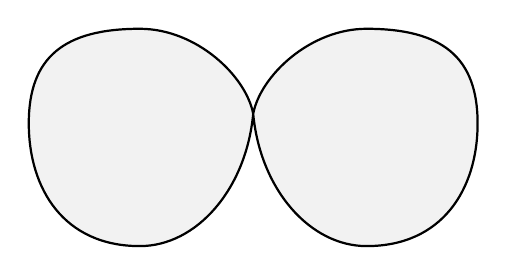
\begin{tikzpicture}[scale=0.6]
            % Create a single smooth path for the merged blob shape using bezier paths
            \draw[thick, fill=gray!10] 
              (0,0.4) 
              .. controls (0.15,-1.2) and (1.2,-2.4) .. (2.4,-2.4) 
              .. controls (4.0,-2.4) and (4.75,-1.2) .. (4.75,0.2) 
              .. controls (4.75,1.6) and (4.0,2.2) .. (2.4,2.2) 
              .. controls (1.2,2.2) and (0.15,1.2) .. (0,0.4)
              
              .. controls (-0.15,-1.2) and (-1.2,-2.4) .. (-2.4,-2.4) 
              .. controls (-4.0,-2.4) and (-4.75,-1.2) .. (-4.75,0.2) 
              .. controls (-4.75,1.6) and (-4.0,2.2) .. (-2.4,2.2) 
              .. controls (-1.2,2.2) and (-0.15,1.2) .. (0,0.4);
          \end{tikzpicture}
          \caption{}
          \label{fig:double_torus}
        \end{subfigure}
        \caption{Note that in this case (and for some equivalence classes), all vertices of a polygon are equivalent by transitivity.}
        \label{fig:polygon}
      \end{figure}
    \end{theorem}

